\subsection{Berechnung des Massendurchsatzes}

Zur Bestimmung des Massendurchsatzes wird die Gleichung \ref{eqn:masse} verwendet. Die Summe der Wärmekapazitäten lässt sich hier 
direkt als $m_2c_{\symup{w}}+m_{\symup{k}}c_{\symup{k}}=\qty(13150)(\joule\per\kelvin)$ bestimmen.

\begin{figure}
    \centering
    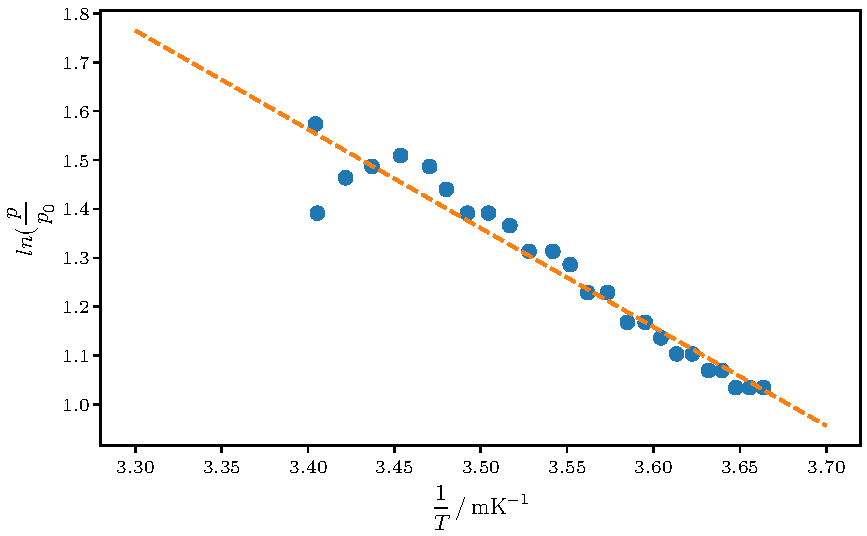
\includegraphics{verdampfplot.pdf}
    \caption{Der Druck bei dem kalten Reservoir gegen dessen Temparatur.}
    \label{fig:druckkalt}
\end{figure}